{\chapter{Background}
\label{chap:Background}

In this chapter, we present the necessary background knowledge concerning topics covered in this thesis. This chapter is consisted of the following sections: 

\begin{itemize}  
\item\textbf{Graphs:}\\
In (\ref{sec:Graphs}), we make a definition for a graph according to the graph theory and discuss the different graph types.

\item \textbf{Graph Data Models:}\\
In (\ref{sec:GraphModels}), we discuss the property graph model (PGM) and the resource description framework model (RDF), as two types of logical graph data models that are mostly used by state of the art graph databases.

\item \textbf{Graph Data Structures:}\\
We present the data structures used by graph databases for the storage of graphs in (\ref{sec:StorageStructures}).

\item \textbf{ Data Structures in C++:}\\
We present necessary background knowledge on a set of $C++$ data structures in (\ref{sec:DataStructuresInC++}).

\item \textbf{Summary:}\\
Lastly, we make a summary of the main topics we discussed in this chapter in (\ref{sec:BackgroundSummary}).
\end{itemize}

\section{Graphs}
\label{sec:Graphs}
In this section, we discuss graphs and graph  types. In (\ref{subsec:Graph?}), we adopt a clear definition for graphs. A definition that is based on the graph theory. In (\ref{subsec:GraphTypes}), we state the different types of graphs. A graph type is a factor that must be taken into consideration in the storage and retrieval methods of the graph.

\subsection{What is a Graph?}
\label{subsec:Graph?}
Graph theory is a mathematical topic that is focused on the study of graphs. A graph \textit{G = (V,E)} is defined as a finite nonempty set \textit{V} of vertices along with the set \textit{E} of edges. The set \textit{E} consists of unordered pairs of vertices in \textit{V}, where an edge \textit{x \(\in\) E} is defined as a pair of vertices \(\textit{x = \{u,v\}}\) \cite{harary6graph}.

We define any two vertices $u \in V$ and $v \in V$ that forms any of the edges in \textit{E} as adjacent vertices. Similarly, two edges $x \in E$ and $y \in E$ are adjacent if they are formed of two pair of vertices where the two pair are sharing one common vertex. The adjacencies of a vertex \textit{u}, is the set $K \subset V$ of vertices, where for each vertex $a \in K$, there is an edge \mbox{$s \in E$} and \textit{s = \{u,a\}} \cite{harary6graph}.

\begin{figure}
\centering
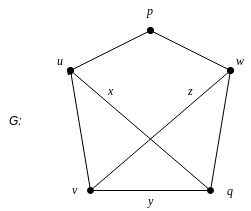
\includegraphics[width=10cm]{pics/Graph.png}
\caption{An example of a graph \textit{G} \cite{harary6graph}.}
\label{fig:graph}
\end{figure} 

In (\ref{fig:graph}), we are showing an example of a graph \textit{G}. In graph \textit{G}, vertices \textit{u} and \textit{v} are adjacent while vertices \textit{u} and \textit{w} are not. Similarly, edges \textit{x} and \textit{y} are adjacent while edges \textit{x} and \textit{z} are not. The adjacencies of vertex \textit{u} in the graph is the set of vertices \textit{\{p,v,q\}} \cite{harary6graph}.




\subsection{Graph Types}
\label{subsec:GraphTypes}

Graphs come in many types and shapes according to how rich they are with information. In (\ref{fig:graph-types}), we show an example of different graph types. A short explanation of each graph type is included in the below list. Some of the below mentioned graph types can be be used together to form one graph \cite{DBLP:journals/corr/abs-1006-2361}.
\\
\\

\begin{figure}
\centering
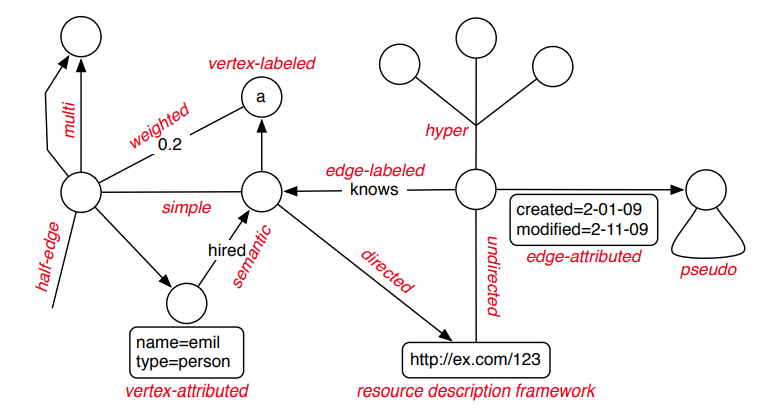
\includegraphics[width=17cm]{pics/graph-types.png}
\caption{An example of different graph types \cite{DBLP:journals/corr/abs-1006-2361}.}
\label{fig:graph-types}
\end{figure} 

\begin{itemize}  
\item \textbf{Simple Graph:} a graph that permits no loops and only binary edges are allowed.

\item \textbf{Multi-graph:} a graph that allows the existence of more than one edge connecting the same two vertices.

\item \textbf{Pseudo Graph:} a graph with reflexive edges

\item \textbf{Weighted Graph:} a graph where a weight is assigned to edges to show the relationship strength.

\item \textbf{Semantic Graph:} used in semantic networks to model the relationships between concepts.

\item \textbf{Half-edge Graph:} an edge that is connected at one of its two ends to a vertex and on the other end connected to nothing.

\item \textbf{Hyper-graph:} a graph that permits an edge to connect more than one vertex.

\item \textbf{Directed Graph:} a graph where each edge is defined by an ordered pair of vertices (one of them is a source vertex and the other is a target vertex).

\item \textbf{Undirected Graph:} a graph where edges are denoting symmetric relationships between edges.

\item \textbf{Edge-labeled Graph:} a graph where edges are identified using a unique edge label or id.

\item \textbf{Vertex-labeled Graph:} a graph where vertices are identified using a unique vertex label or id.

\item \textbf{Edge-attributed Graph:} a graph where descriptive properties are assigned to edges.

\item \textbf{Vertex-attributed Graph:} a graph where descriptive properties are assigned to vertices.

\item \textbf{Resource Description Framework (RDF) Graph:} a graph where vertices and edges are identified by Uniform Resource Identifiers (URI). The RDF is a standard that was issued by the World Wide Web consortium.

\end{itemize}


\section{Graph Data Models}
\label{sec:GraphModels}

In (\ref{sec:Graphs}), we presented the definition of graph and introduced the difference between the various graph types. In this section, we discuss two logical graph data models. First, we present the property graph model (PGM) in (\ref{subsec:PGM}). Next, we present the resource description framework model (RDF) in (\ref{subsec:RDF}).


\begin{figure}[H]
\centering
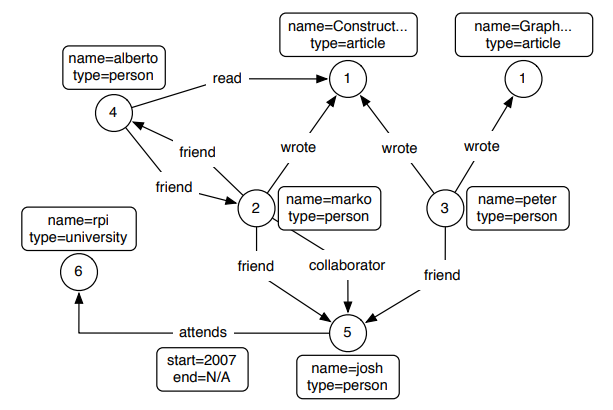
\includegraphics[width=17cm]{pics/PGM.png}
\caption{A diagram of a property graph \cite{DBLP:journals/corr/abs-1006-2361}.}
\label{fig:PGM}
\end{figure} 

\subsection{Property Graph Model}
\label{subsec:PGM}

Several graph database systems are supporting the property graph model. The property graph model is characterized with being directed, labeled, attributed and multi-graph. In (\ref{fig:PGM}), we show an example diagram of a property graph model. 

In property graph model, an edge is defined as an ordered pair of vertices. The first vertex in the pair is the source vertex of the edge and the second vertex in the pair is the target vertex of the edge. 

Vertices and edges in a property graph model are labeled. A vertex label is an identifier for the vertex while an edge label is used to define the relationship type of an edge. 

A vertex in the property graph model is described by properties (or attributes). The properties describing a vertex are a set of key-value pairs. An example of a property describing a vertex in (\ref{fig:PGM}) is \textit{"name"="alberto"} property which is describing vertex "4". Similarly, an edge can also be described by a set of key-value properties. An example of a property describing an edge in (\ref{fig:PGM}) is \textit{"start"="2007"} property which is describing edge "attends".

Property graph model is supporting also the creation of multi-graphs. In a multi-graph, more than two edges can be defined using the same pair of vertices and with the same direction, given that the edges have different labels \cite{DBLP:journals/corr/abs-1006-2361, Robinson:2015:GDN:2846367}.



\subsection{Resource Description Framework Model (RDF)}
\label{subsec:RDF}

The World Wide Web consortium (W3C) has developed the Resource Description Framework (RDF) as a foundation for metadata exchanging and processing across the web. RDF is used mostly in building semantic webs. The RDF standard is used to express the metadata of the web documents. RDF is well supported by a model of triples. A triple is consisting of a resource, a property, and a value. The RDF model is characterized with being a vertex-labeled, edge-labeled, and directed graph \cite{ngomo2014introduction}.

A resource is anything that can be uniquely identified using a Unique Resource Identifier (URI). A web page is an example of a resource identified by its Unique Resource Locator (URL). A property is used to define a binary relationship between a resource and a value. A value itself can be a resource or a string of characters. A triple is considered as an RDF statement that is defined by the three elements (resource, property, value) \cite{Las99,Lee2005}.



In (\ref{fig:RDF}), we show an example of an RDF graph that is consisting of 9 triples. The graph is describing the city of Leipzig and its mayor. An example of a triple in the graph is \textit{("Leipzig", "locatedIn", "Saxony")} with \textit{"Leipzig"} representing the resource, \textit{"locatedIn"} representing the property, and \textit{"Saxony"} representing the value in the triple.


\begin{figure}[H]
\centering
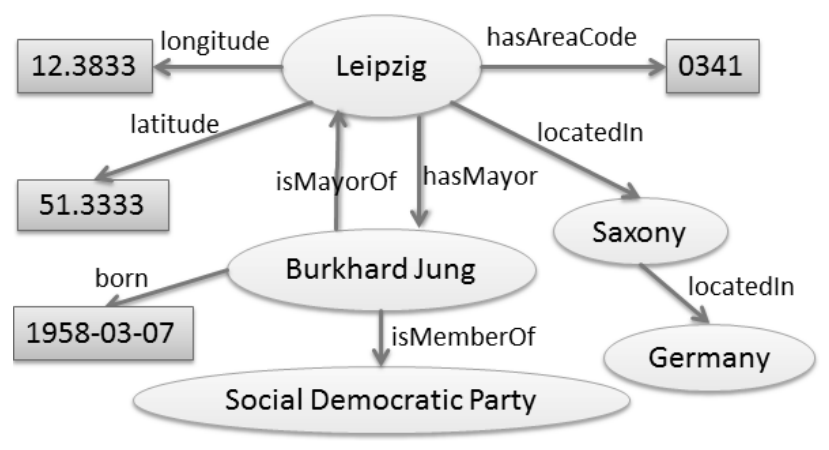
\includegraphics[width=15cm]{pics/RDF-Graph.png}
\caption{An example of an RDF graph that consists of 9 triples \cite{ngomo2014introduction}.}
\label{fig:RDF}
\end{figure} 

\section{Graph Data Structures}
\label{sec:StorageStructures}

In (\ref{sec:GraphModels}), we presented two logical graph data models. First, we presented the property graph model (PGM) in (\ref{subsec:PGM}). Next, we presented the resource description framework model (RDF) in (\ref{subsec:RDF}). In \cite{Paradies2017},  the authors (\textit{Paradies et al.}) categorized the data structures used to store graph data into two categories. First category is for the graph data structures used by graph databases for solely storing a directed graph topology. Second category is for the graph data structures used by graph databases for solely storing graph properties. In this section, we adopt the categorization presented in \cite{Paradies2017} and present the necessary background information of a selected subset of graph data structures. We first discuss three data structures (Adjacency Matrix, Compressed Sparse Row (CSR), Adjacency List) for graph topology in (\ref{subsec:GraphTopology}). Next, we present three data structures (Universal Table, Emerging Schema, Nested Key-Value Store) for storing graph properties in (\ref{subsec:GraphProperties}).


\subsection{Graph Topology}
\label{subsec:GraphTopology}

The graph topology storage structures are meant to store the topology of a graph. We mean by the topology of a graph, the vertices of the graph identified by their labels and the directed edges connecting those vertices, leaving out the edge-labels, vertex-properties and edge-properties.

In this section, we introduce three data structures that can be utilized by graph databases for the storage of a graph topology. In (\ref{subsubsec:AdjacencyMatrix}), we present the adjacency matrix as the first storage structure for graph topology. Next, we present the compressed sparse row (CSR) in (\ref{subsubsec:CSR}). Lastly, we present the adjacency list in (\ref{subsubsec:AdjacencyList}).


\begin{figure}[H]
\centering
    \subfigure[Directed graph \textit{G}.]
    {
        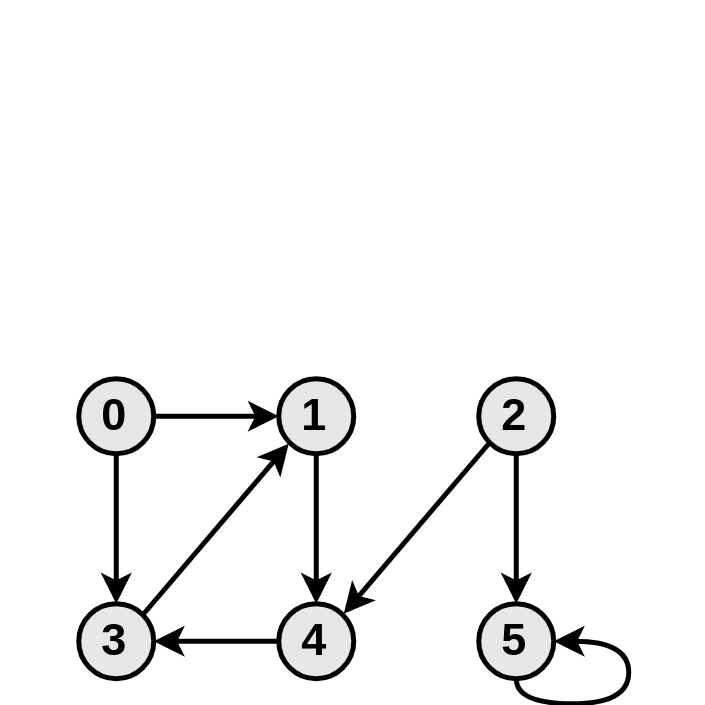
\includegraphics[width=0.35\textwidth]{pics/DirectedGraph.png}
        \label{fig:directedGraph_logical}
    }
\centering
    \subfigure[Adjacency matrix representation of \textit{G}.]
    {
        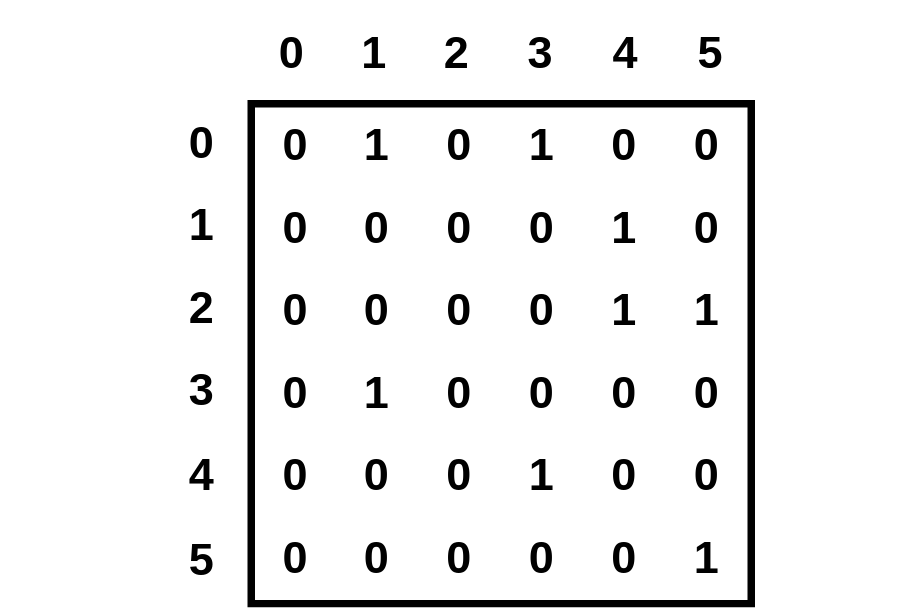
\includegraphics[width=0.42\textwidth]{pics/AdjacencyMatrix_logical.png}
        \label{fig:adjMat_logical}
    }
    \\
\centering
    \subfigure[CSR representation of \textit{G}.]
    {
        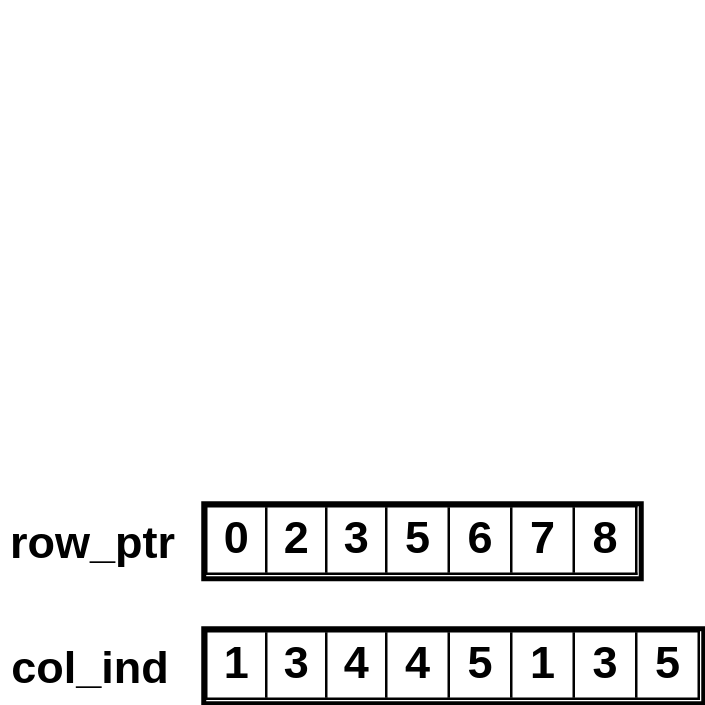
\includegraphics[width=0.35\textwidth]{pics/CSR_logical.png}
        \label{fig:CSR_logical}
    }
    \subfigure[Adjacency list representation of \textit{G}.]
    {
        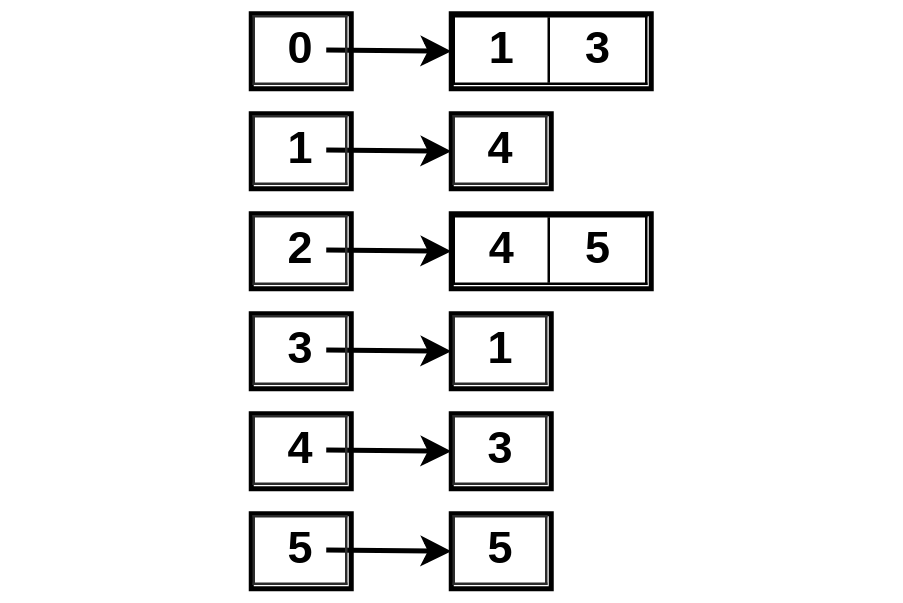
\includegraphics[width=0.4\textwidth]{pics/AdjacencyList_logical.png}
        \label{fig:adjLst_logical}
    }
    \caption{Logical representations of the topology of directed graph \textit{G} \cite{cormen2009introduction}.}
    \label{fig:GraphTopology_logical}
\end{figure}


\subsubsection{Adjacency Matrix}
\label{subsubsec:AdjacencyMatrix}

The adjacency matrix is the preferred method of storing graph \textit{G = (V,E)} when the graph is dense (i.e. \textit{$|E| \approx |V|^2$}) or in case there is a need to get a fast response on checking for two vertices \textit{u} and \textit{v}, if there is an edge tying them to each other. 

For a directed graph \textit{G = (V,E)}, the adjacency matrix \textit{A} representing the graph is a \textit{$|V| \times |V|$} matrix and the vertices of the graph are labeled with a sequence of numbers 1,2,...,\textit{|V|}. For a cell \textit{$a_{ij}$} in matrix \textit{A} where \textit{$1 \leq i \leq |V|$} and similarly \textit{$1 \leq j \leq |V|$}, a value of "1" is assigned to the cell if \textit{(i,j) \(\in\) E}, otherwise, a value of "0" is assigned to the cell \cite{cormen2009introduction}.

In (Figure \ref{fig:directedGraph_logical}), we show an example of a vertex-labeled directed graph \textit{G} that is consisted of 6 vertices and 8 edges. In (Figure \ref{fig:adjMat_logical}), we show the adjacency matrix logical representation of \textit{G} \cite{cormen2009introduction}. 

The memory required for storing an adjacency matrix of a graph is $O(|V|^2)$ which is not affected by the number of edges \textit{|E|} in the graph \cite{cormen2009introduction}.



\subsubsection{Compressed Sparse Row (CSR)}
\label{subsubsec:CSR}

Sparseness of an adjacency matrix \textit{A} can be solved by storing only the non-zero elements of the matrix (i.e. recording only the existence of an edge and discarding information about the absence of an edge between two vertices). The compressed sparse row (CSR) is a compact storage format that stores only non-zero elements of a sparse matrix. The compressed sparse row (CSR) format is storing the information about the non-zero elements of the matrix in two vectors with contiguous memory locations \textit{(col\_ind,row\_ptr)}. We store the column indices of the non-zero elements in the matrix in \textit{col\_ind} ordered by their position precedence in the matrix when scanning the matrix in a row-wise left-to-right traversal. In \textit{row\_ptr}, we store only the indices of the elements in \textit{col\_ind} that are located first in their respective rows in the matrix \cite{Bai:2000:TSA:357352,Paradies2017}.

In (Figure \ref{fig:CSR_logical}), we show the compressed sparse row (CSR) that is representing the adjacency matrix in (Figure \ref{fig:adjMat_logical}) and consequently representing the vertex-labeled directed graph \textit{G} in (Figure \ref{fig:directedGraph_logical}) \cite{Bai:2000:TSA:357352}.

Instead of storing $|V|^2$ elements in the adjacency matrix, the compressed sparse row (CSR) format is consuming much less storage by storing only $nnz + |V| + 1$ elements, where $nnz$ is the number of non-zero elements in the matrix \cite{Bai:2000:TSA:357352}. Although the compressed sparse row (CSR) format is offering a contiguous memory allocation of the graph data compacted in two vectors, a manipulation by adding or removing elements to CSR is expensive. Because the order of elements stored in the two vectors \textit{(col\_ind,row\_ptr)} must always be maintained, a manipulation to the CSR data implies a reorganization of the elements in the vectors to maintain their elements order.

\subsubsection{Adjacency List}
\label{subsubsec:AdjacencyList}

In adjacency matrix we faced the problem of storing redundant and unnecessary information regarding the absent edges. Although the compressed sparse row (CSR) format has offered a solution to this problem by storing only the necessary information, it raised a different issue which is the expensive manipulation of the data.

The adjacency list \textit{Adj} of a graph \textit{G = (V,E)} is composed of a set of $|V|$ pairs. Each pair is consisted of a vertex $u$ and a vector $K$ that contains the adjacencies of $u$ \cite{van1998python}.

Adjacency lists is memory efficient in storing sparse graphs by storing only information that indicates the existence of an edge. Adjacency lists keeps the adjacencies vector $K$ of each vertex ordered for efficient look-up operations. Adding or removing a vertex to/from $K$ requires a reorganization of the elements in the vector to maintain the elements order. The overhead of reorganizing the elements in $K$ is proportional to the size of $K$ which is less when compared to the similar overhead in CSRs that is proportional to $|V|$ \cite{van1998python}.

In (Figure \ref{fig:directedGraph_logical}), we show an example of a vertex-labeled directed graph \textit{G} that is consisted of 6 vertices and 8 edges. In (Figure \ref{fig:adjLst_logical}), we show the adjacency list logical representation of \textit{G} \cite{cormen2009introduction}. 

The memory required for storing an adjacency list of a graph is $O(|V| + |E|)$ \cite{cormen2009introduction}.







\begin{figure}[H]
\centering
    \subfigure[An attributed directed graph \textit{G} \cite{DBLP:journals/corr/ParadiesLB14}.]
    {
        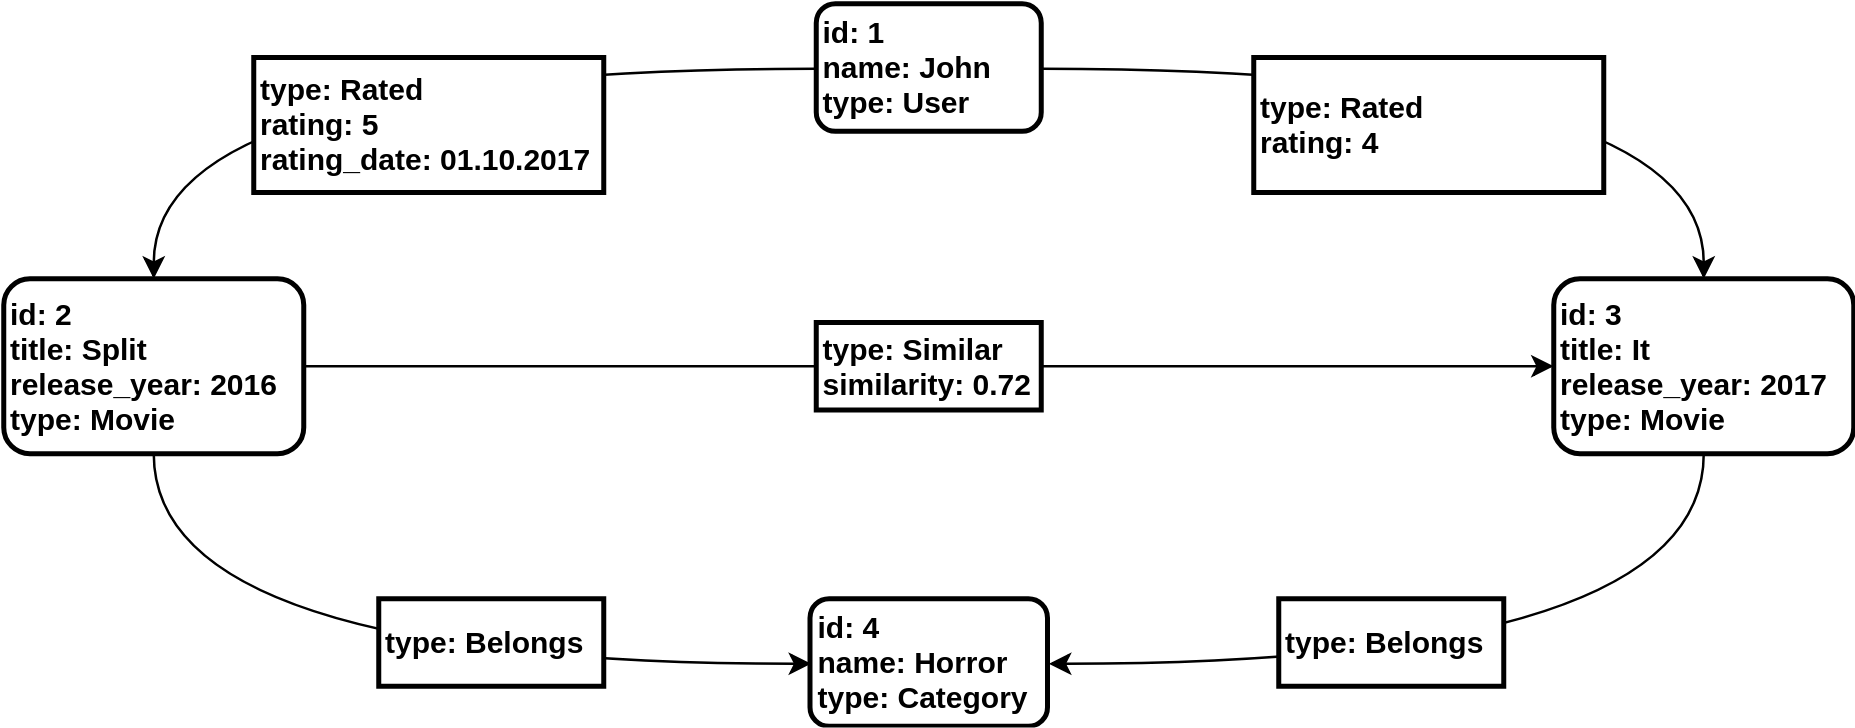
\includegraphics[width=1\textwidth]{pics/PropertyGraph.png}
        \label{fig:PropertyGraph}
    }
\centering
    \subfigure[Vertex universal table of \textit{G} \cite{DBLP:journals/corr/ParadiesLB14}.]
    {
        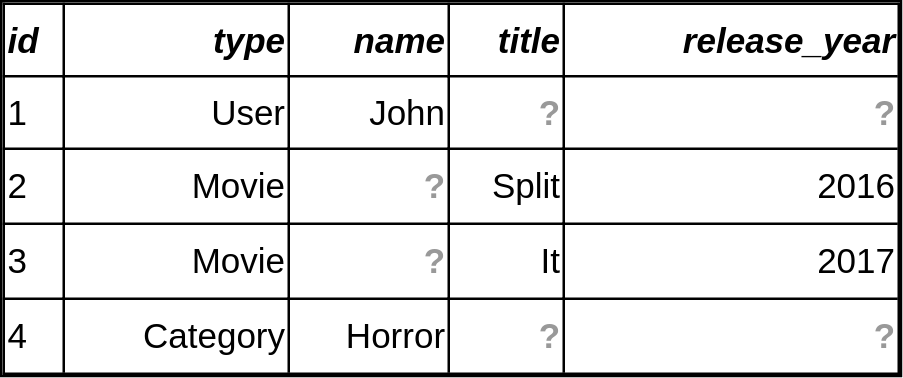
\includegraphics[width=0.45\textwidth]{pics/VertexUniversalTable.png}
        \label{fig:VertexUniTbl}
    }
\centering
    \subfigure[Edge universal table of \textit{G} \cite{DBLP:journals/corr/ParadiesLB14}.]
    {
        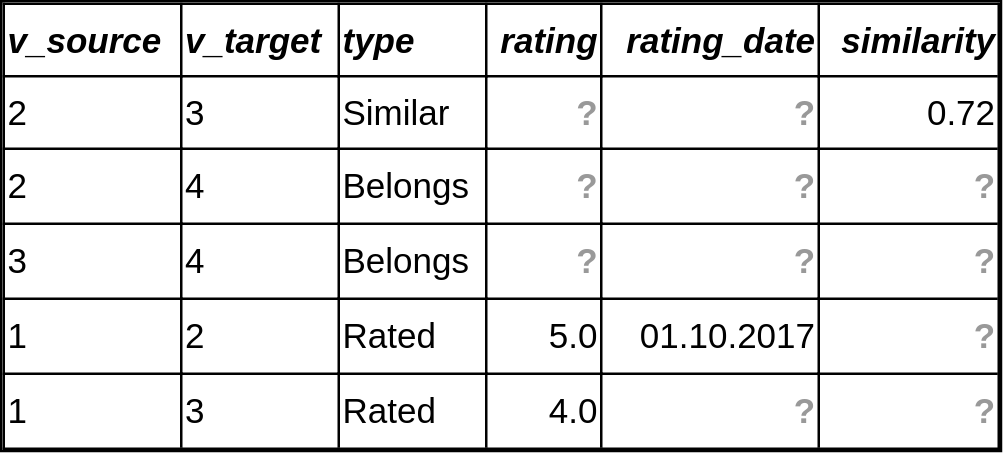
\includegraphics[width=0.5\textwidth]{pics/EdgeUniversalTable.png}
        \label{fig:EdgeUniTbl}
    }
\centering
    \subfigure[Emerging Schema - vertex column groups of \textit{G}.]
    {
        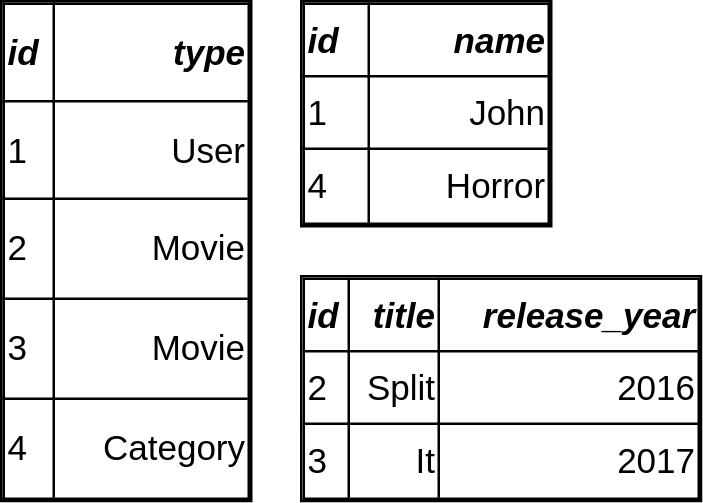
\includegraphics[width=0.45\textwidth]{pics/VertexEmergingSchema.png}
        \label{fig:VertexEmergingSchema}
    }
\centering
    \subfigure[Emerging Schema - edge column groups of \textit{G}.]
    {
        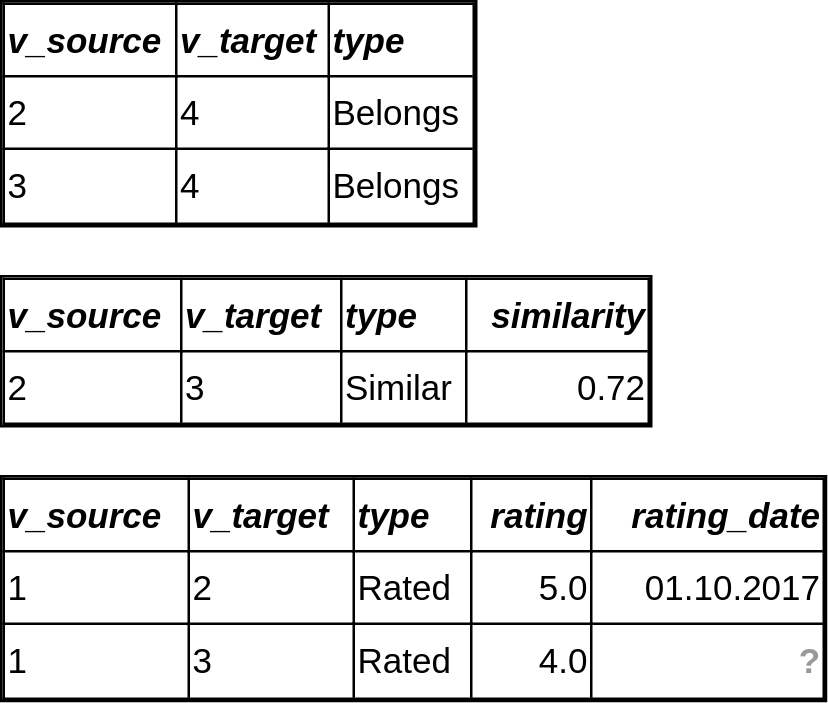
\includegraphics[width=0.5\textwidth]{pics/EdgeEmergingSchema.png}
        \label{fig:EdgeEmergingSchema}
    }
    \caption{Universal table and emerging schema representations of property graph \textit{G}.}
    \label{fig:GraphProperties_logical}
\end{figure}

\subsection{Graph Properties}
\label{subsec:GraphProperties}

In (\ref{subsec:GraphTopology}), we introduced three graph topology data structures. The three data structures are storing information only regarding the graph topology, leaving out the storage of information regarding the properties of the graph to the graph properties data structures. 

In this section, we introduce three data structures that can be utilized by graph databases for storing the properties of vertices and edges for a given graph. In (\ref{subsubsec:UniversalTable}), we present the universal table. Next, we present the emerging schema approach in (\ref{subsubsec:EmergingSchema}). Lastly, we present the nested key-value store in (\ref{subsubsec:NestedkeyValueStore}).

\subsubsection{Universal Table}
\label{subsubsec:UniversalTable}

Universal tables is a method of storing the vertices and edges properties in only two tables. Each object (vertex or edge) is represented by a single row in the respective universal table. A column in the universal table is representing a distinct object's property. A null value in in the universal table means that the property represented by the referenced column is not applicable to that object stored in the respective row \cite{Paradies2017}.

Vertices and edges can have a high number of distinct properties, where only a few of those properties are applicable to a specific vertex or edge. The in-applicability of all properties to all vertices or edges leads to a degree of sparseness in universal table. Sparseness can be a problem in storing large graphs by consuming more memory. However, the storage of an object (vertex or edge) in a single row allows for a join-free method to extract an object's properties \cite{Paradies2017}.

In (Figure \ref{fig:PropertyGraph}), we show an example of an attributed directed graph $G$ that is composed of 4 vertices and 5 edges. In (Figure \ref{fig:VertexUniTbl}), we show a vertex universal table representing $G$, where each single vertex in $G$ is represented by a single row and each distinct vertex property is represented by a separate column. Similarly, in (Figure \ref{fig:EdgeUniTbl}), we show an edge universal table of $G$, where each single edge in $G$ is represented by a single row and each distinct edge property is represented by a separate column. Question marks in the tables denotes absence of a value (i.e. a null value) \cite{Paradies2017}.


\subsubsection{Emerging Schema}
\label{subsubsec:EmergingSchema}

In (\ref{subsubsec:UniversalTable}), we discussed a simple method of storing an attributed graph using only a pair of universal tables, a vertex universal table and an edge universal table. The universal table method is subject to a drawback as it tends to be more sparse as the number of distinct properties increase.

Emerging schema is a method that applies vertical partitioning on the properties of objects (vertices or edges) in a way that reduces the sparseness of the data stored and at the same time doesn't require the joining of many tables to extract a single object's properties. The emerging schema method is exploiting the inherent schema of the data to create a set of column groups for vertices and another set of column groups for edges. 

Each column group is consisted of multiple columns where the first column is always representing the unique object's label. In addition to the object's label column, properties that co-occur frequently together are clustered into the same column group. An object can be represented by a row in one or more of the column groups. An object is represented by a row in a specific column group, only if the object has at least one property represented by a column in the respective column group. Objects with no descriptive properties are grouped together into a default column group \cite{Paradies2017}.

The clustering of properties into column groups can be done by applying machine learning clustering algorithms such as k-means on the data in the universal table \cite{macqueen1967,Paradies2017}. The input to the clustering algorithm is the data stored in the universal table. Each column in the universal table is considered an $n-dimension$ point provided to the clustering algorithm, where $n$ is the number of rows in the table and the value for each dimension is "1" in case a non-null value and "0" in case of a null value. 

Clustering is applied once on the vertex universal table and once on the edge universal table. A single object's (vertex or edge) row is constructed from the resulted column groups by joining them over the object-label column.

In (Figure \ref{fig:PropertyGraph}), we show an example of an attributed directed graph $G$ that is composed of 4 vertices and 5 edges. In (Figure \ref{fig:VertexEmergingSchema}), we present the vertex column groups for $G$ that is produced by the emerging schema method. Similarly, in (Figure \ref{fig:EdgeEmergingSchema}), we present the edge column groups for $G$ that is produced by the emerging schema method. Question marks in the column groups denotes absence of a value (i.e. a null value) \cite{Paradies2017}. 

Even though graph $G$ is attributed, it is not explicitly defining an identifying label for each object. For storing the graph data in a universal table, an identifying label must be defined for each vertex and edge. The property $"id"$ that describes the vertices is appearing to have a unique value for each vertex and hence we used it to act as the vertex-label. For edges, we found three properties that we can use to uniquely identify each edge. The three properties are the $"id"$ property of the source vertex, the $"id"$ property of the target vertex, and the $"type"$ property of an edge. The concatenation of the three properties is acting as the edge-label.


\subsubsection{Nested Key-Value Store}
\label{subsubsec:NestedkeyValueStore}

In this section, we are presenting another approach for solving the sparseness problem of universal tables we discussed in (\ref{subsubsec:UniversalTable}).

Graph properties are composed of vertices-properties and edges-properties. The properties of an object (vertex or edge) are consisted of key-value pairs that describe the object. In a given vertex-attributed and edge-attributed graph $G = (V,E)$, for each vertex $u \in V$ and edge $x \in E$, a set $P$ of key-value pairs exists. Each key-value pair $(k,v) \in P$, is consisted of a property $k$ that describes the object and a value $v$ that is assigned to $k$ \cite{ladwig2011cumulusrdf}.

Nested key-value stores are storing an object's properties in a two level nested key-value stores. The first level of the store is representing rows, where each object is stored in a row. The object's row is represented by a key-value pair, where the key is the object-label and the value is itself a second level of a key-value store. The key-value store on the second level is to represent columns, where each object's property is stored in a column. Each column is represented by a key-value pair, where the key is the name of the property describing the object and the value is a string of characters \cite{ladwig2011cumulusrdf}.

Sparseness problem of universal tables is eliminated in the nested key-value store by storing only the values for the properties that are applicable for a given vertex or edge. In this way, the size of the second level of key-value store for each row is equal to the number of non-empty properties describing the respective vertex or edge. We store the properties of the vertices in one nested key-value store separated from another nested key-value store that we use for the storing the edges properties.


\begin{figure}[t]
\centering
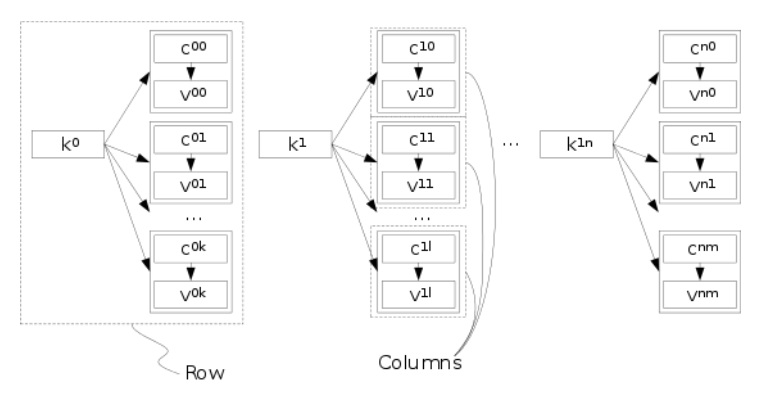
\includegraphics[width=15cm]{pics/NestedKey-ValueStore.png}
\caption{A nested key-value store composed of rows and columns \cite{ladwig2011cumulusrdf}.}
\label{fig:nestedKey-ValueStore}
\end{figure} 

Storing the property name together with its value in the nested key-value store, makes any modifications to the property name needs to be applied to each row in the entire nested key-value store. Also, as the sparseness of the data represented in the universal table is decreased, the memory requirements to store the property name redundantly in every row will increase.

In (\ref{fig:nestedKey-ValueStore}), we show a diagram of a nested key-value store that is composed of rows and columns. On the first level of the store, rows are stored, while columns are stored in the second level of the store \cite{ladwig2011cumulusrdf}.

The nested key-value store is searched for an object's row using the object-label $(k)$ and the value returned is the object's columns $(c)$. The object's columns $(c)$ are searched for a specific column or property to return the value $(v)$ of that column \cite{ladwig2011cumulusrdf}.




\section{Data Structures in C++}
\label{sec:DataStructuresInC++}

In (\ref{sec:StorageStructures}), we discussed the logical design of graph data structures. In this section, we present necessary background knowledge on data structures offered as part of the \textit{Standard Template Library} (STL) of the $C++$ programming language. In (\ref{chap:PhysicalDesign}), we will use the data structures presented in this section as the building blocks for the physical design of graph data structures.

We will start with introducing the (\texttt{std::vector}) data structure in (\ref{subsec:vector}). Next, we present the (\texttt{std::map}) data structure in (\ref{subsec:map}). In (\ref{subsec:unorderedmap}), we present the (\texttt{std::unordered\_map}) data structure. Lastly, we present the (\texttt{std::pair}) data structure in (\ref{subsec:pair}).

\subsection{\texttt{std::vector}}
\label{subsec:vector}

The (\texttt{std::vector}) data structure is a sequence container that is offered as part of the $STL$ library in the $C++$ programming language. Sequence containers are storing their elements in contagious memory locations \cite{josuttis2012c++}.

Elements stored in a (\texttt{std::vector}) are atomic values of the same type.The order of the elements in the (\texttt{std::vector}) is the same as the order of inserting them into the container if they are appended to the end of the (\texttt{std::vector}). Another way to control the order of the elements is to insert them at exact positions in the (\texttt{std::vector}). The value of the element doesn't affect the order of the element in the container \cite{josuttis2012c++}. 

The (\texttt{std::vector}) data structure is usually implemented as a dynamic array that can grow and shrink in size. Appending elements to the end of the (\texttt{std::vector}) is very fast as it takes a constant time with a complexity of $O(1)$. Inserting element at any other position than the end of the (\texttt{std::vector}) takes more time, as all the following elements need to be displaced to free room for the inserted element. The complexity of the insertion at a position other than the end is linear $O(n)$.  Accessing an elements in a (\texttt{std::vector}) by position is so fast as it takes a constant time $O(1)$, while the complexity of finding an element in a (\texttt{std::vector}) using the element's value is linear to the size of the (\texttt{std::vector}) \cite{josuttis2012c++}.

\subsection{\texttt{std::map}}
\label{subsec:map}

The (\texttt{std::map}) data structure is an associative container that is offered as part of the $STL$ library in the $C++$ programming language. Elements in an associative container are accessed using their values rather than their position in the container \cite{josuttis2012c++}.

An element in a (\texttt{std::map}) container is consisted of a key-value pair where the key of each pair is unique in the entire (\texttt{std::map}). The key and value which together are forming an element in a (\texttt{std::map}) can be of different types. Elements in a (\texttt{std::map}) are sorted by their keys according to the compactor of the stored elements data type. The order of insertion has no effect on the order of the elements in the container. 

Storing the elements in a (\texttt{std::map}) sorted by their keys allows for range queries to be performed on the elements stored in the container \cite{josuttis2012c++}. 

The (\texttt{std::map}) data structure is usually implemented as a binary search tree. Insertion of a new element or finding an existing one in a (\texttt{std::map}) has a logarithmic complexity $O(log(n))$ where "$n$" is the number of elements in the (\texttt{std::map}). Modifying the key of an element in a (\texttt{std::map}) can't be done as it will invalidate the order of the elements in the container. Instead, the element has to be removed and inserted again with the new key \cite{josuttis2012c++}.

\subsection{\texttt{std::unordered\_map}}
\label{subsec:unorderedmap}

The (\texttt{std::unordered\_map}) data structure is an associative container that is offered as part of the $STL$ library in the $C++$ programming language. Elements in an associative container are accessed using their values rather than their position in the container \cite{josuttis2012c++}.

Similar to the (\texttt{std::map}) data structure, an element in a (\texttt{std::unordered\_map}) container is consisted of a key-value pair where the key of each pair is unique in the entire (\texttt{std::unordered\_map}). The key and value which together are forming an element in a (\texttt{std::unordered\_map}) can be of different types. In contrast to the (\texttt{std::map}) data structure, elements in a (\texttt{std::unordered\_map}) don't have any defined order. The order of insertion has no effect on the order of the elements in the container nether the elements' values \cite{josuttis2012c++}. 

The (\texttt{std::unordered\_map}) data structure is usually implemented as a hash-table. The hash-table is consisted of buckets where each element in the container is stored in a specific bucket depending on a hash value that is determined by a special hash function. Finding an element by its value in a (\texttt{std::unordered\_map}) container has a constant time complexity of $O(1)$. A feature of a good hash function is that it generates hash values to all the available buckets in the container. Growing the size of a (\texttt{std::unordered\_map}) data structure requires a rehashing to all the elements that are already stored in the container. Using the hash function, a rehashing of an element is done by generating a new hash value for the element to determine the element's new location in the container \cite{josuttis2012c++}.


\subsection{\texttt{std::pair}}
\label{subsec:pair}

The (\texttt{std::pair}) data structure is a simple container that is offered in the $C++$ programming language. A (\texttt{std::pair}) structure is offering the storage of two values of different types as a single unit. The two values stored in a (\texttt{std::pair}) have a concrete order. A value is accessed in the (\texttt{std::pair}) by specifying the value's position in the structure whether it is the first or the second \cite{josuttis2012c++}.

\section{Summary}
\label{sec:BackgroundSummary}

In this chapter, we made a formal definition of a graph according to the graph theory and discussed the different graph types. We presented two logical graph models that are most commonly used  by state of the art graph databases, the property graph model (PGM) and the resource description framework model (RDF). We presented several storage structures used by graph databases to store graph data and we differentiated between structures used to store graph topology and structures used to store graph properties. We presented a set of data structures that are offered by the $C++$ programming language which we will use as the building blocks for the physical design of graph data structures.

Aiming to evaluate and benchmark the different graph storage structures, we implemented a set of graph storage structures by their two types (graph topology structures and graph properties structures). In the next chapter, we present the details of the implementation with a focus on the physical design of the graph storage structures we implemented.

}